\documentclass[a4paper]{article}

%% Language and font encodings
\usepackage[english]{babel}
\usepackage[utf8x]{inputenc}
\usepackage[T1]{fontenc}

%% Sets page size and margins
\usepackage[a4paper,top=3cm,bottom=2cm,left=3cm,right=3cm,marginparwidth=1.75cm]{geometry}

%% Useful packages
\usepackage{amsmath}
\usepackage{amssymb}
\usepackage{graphicx}
\usepackage[colorinlistoftodos]{todonotes}
\usepackage[colorlinks=true, allcolors=blue]{hyperref}

\usepackage{amsthm}
\usepackage {stmaryrd}

\usepackage{listings}
\usepackage{color}

\definecolor{dkgreen}{rgb}{0,0.6,0}
\definecolor{gray}{rgb}{0.5,0.5,0.5}
\definecolor{mauve}{rgb}{0.58,0,0.82}

\lstset{language=sql,
  aboveskip=3mm,
  belowskip=3mm,
  showstringspaces=false,
  columns=flexible,
  basicstyle={\small\ttfamily},
  numbers=none,
  numberstyle=\tiny\color{gray},
  keywordstyle=\color{blue},
  commentstyle=\color{dkgreen},
  stringstyle=\color{mauve},
  breaklines=true,
  breakatwhitespace=true,
  tabsize=3
}

\usepackage{tikz}
\usetikzlibrary{automata,positioning}

\theoremstyle{definition}
\newtheorem{Ex}{Exercice}

\title{Spatial modelization of AHL dispersion in a bounded space}
\author{Ardoin, Lichtle, Riou}

\begin{document}
\maketitle

\section*{Introduction}

In this small paper, our aim is to determine the behaviour of bacteria whiwh use quorum sensing to communicate. In particular, we will interest on bacteria which produce N-Acyl homoserine lactone (abbreviated AHL), a signaling molecule whose concentration influences the probability for bacteria to self-destruct. The dispersion of this molecule thus enables bacteria to have a synchronized behaviour, which can have several applications, for instance in medicine.

This paper is mainly inspired by a 2016 paper from Din \textit{et al.} called "Synchronized cycles of bacterial lysis for \textit{in vivo} delivery" which notably proposes a simulation for the behaviour of bacteria using AHL molecules, but without any spatial aspect, considering the density of AHL is uniform in the space.

Thus we added spatial considerations to the existing model, and implemented this more precise simulation, using C++ SFML library in order to visualize the evolution of bacteria population and AHL density.

The complete code of our simulation can be found at the following URL:\\ \texttt{https://github.com/nathanlct/cancer-fighting-bacteria-simulation}

\section{The initial approach: an ideal simulation}

In the paper we base our work on, the simulation was taking place in a cell trap where everything was perfectly mixed, such that the AHL density is uniform. In this way, there is just a general simulation of every concentration to calculate. A periodic pattern appears clearly with such a model.

\begin{figure}[!h]
        \centering
        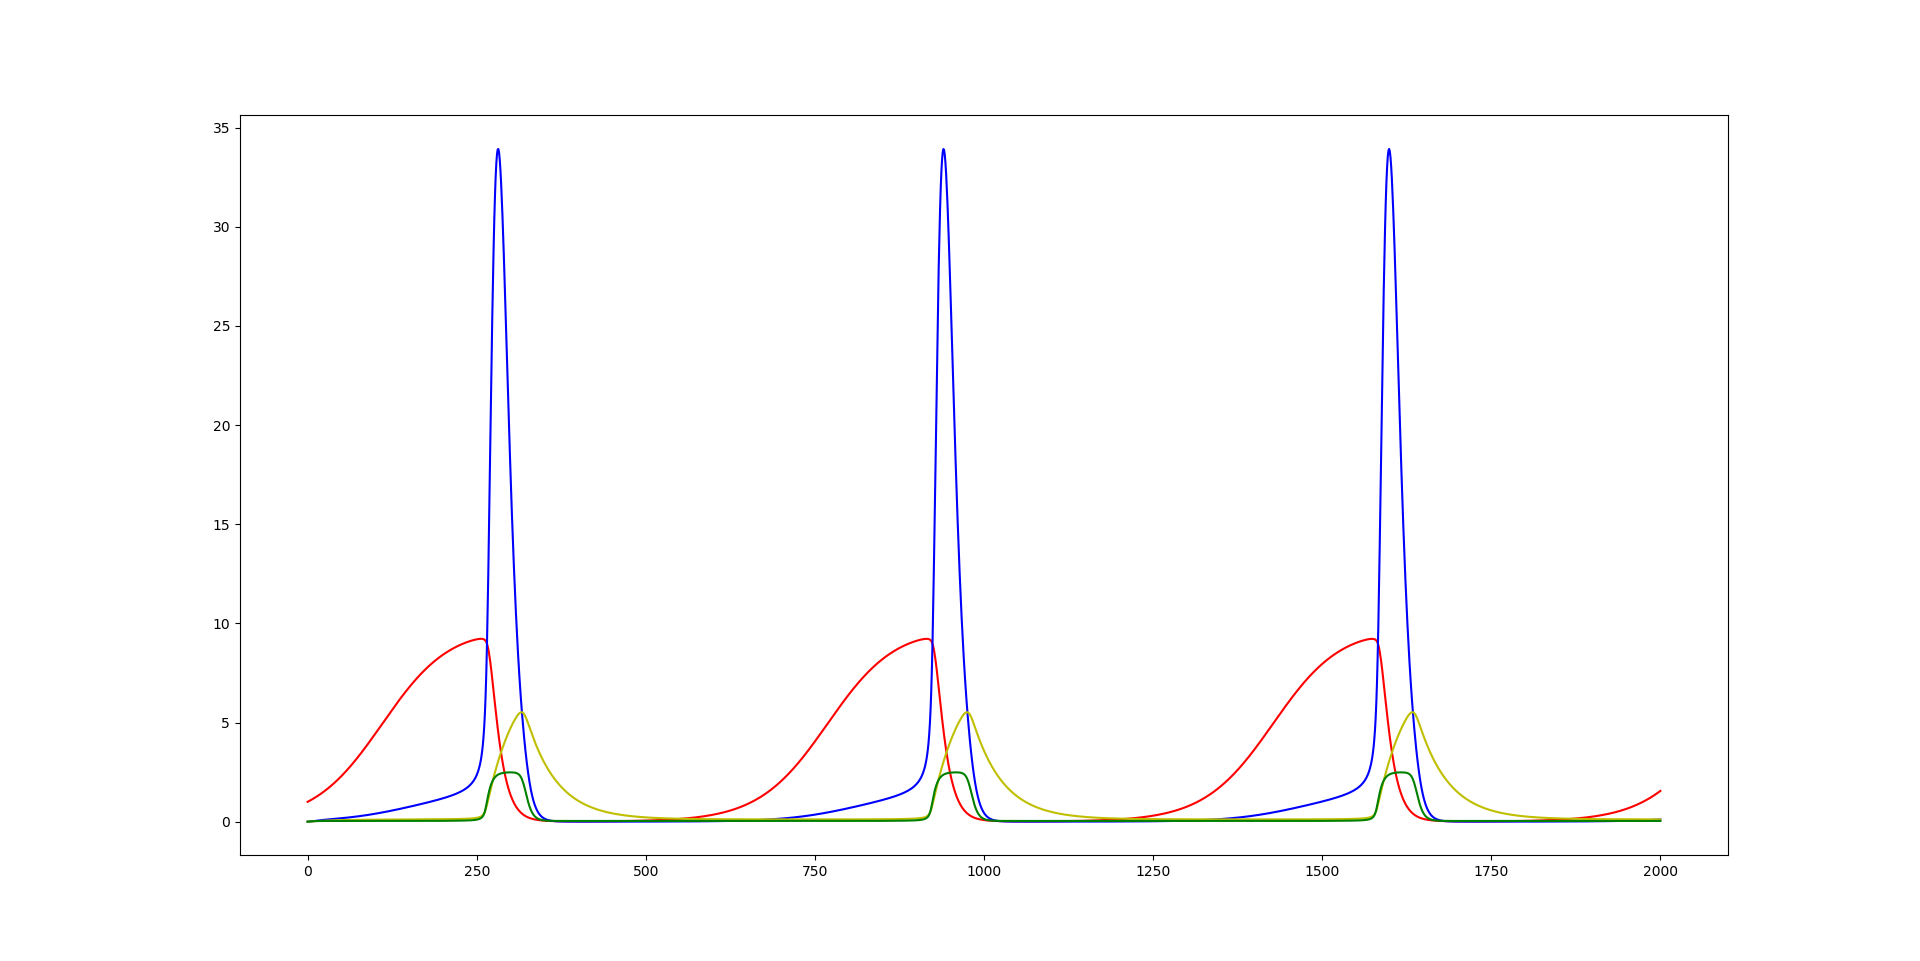
\includegraphics[width=1\textwidth]{Figure_2.png}
        \caption{Plot of the ideal simulation}
\end{figure}

\section{Presentation}

First, we consider that the experience takes place in a bounded metric space $E$.

In this space, some bacteria evolve. A \emph{bacterium} is considered as a material point in space $E$, and we denote $p_n(t)$ the position of bacterium $n$ at time $t$.

Moreover, bacteria produce a plasmid LuxI (denoted $I$) and a lysis protein (denoted $L$). At any time $t$, we denote $I_n(t)$ (resp. $L_n(t)$) the intracellular concentration of LuxI (resp. lysis protein) of bacterium $n$. Bacteria also produces AHL at regular intervals. We denote $H : E \times \mathbb{R}_+ \to \mathbb{R}_+$ the function of AHL density, such that $H(M,t)$ represents the density of AHL on position $M$ at time $t$.

Finally, bacteria are able to do two important actions: \emph{reproduce} themselves and \emph{self-destruct}. Therefore, the set of bacteria is not constant, thus we denote $N_t$ the set of all bacteria which exists in space $E$ at time $t$.

\section{Modelling}

\subsection{Moves of bacteria and AHL particles}

We consider that bacteria move following a brownian movement. In terms of visualization, we thus represent them as spheres of constant radius which move randomly. When any bacterium touches a border of the space, it simply follows the same move but in the symmetric direction. For example, if some bacterium touches a vertical bound while its speed is a vector $(\vec{v}_x, \vec{v}_y)$, its new speed will be $(-\vec{v}_x, \vec{v}_y)$.

TODO collisions cells

We suppose that AHL molecules are very small in comparison with bacteria, therefore we represent these molecules by a function of density defined on all the space $E$. This density depends on the ponctual production of AHL by bacteria, but also evolves temporaly because of the propagation of these molecules in the fluid in which they are produced.

We represent this propagation using convolutions, such that at any time $t$ :
\begin{equation}
\frac{dH}{dt}(x,y,z,t) = (H * g)(x,y,z,t) := \iiint \limits_E H(x-u,y-v,z-w,t)g(u,v,w) du dv dw
\end{equation}
where $g$ is a filter defined on $E$.

Using convolutions to represent a propagation of our signal is inspired from classical algorithms of image processing. Intuitively, the idea is to choose a well defined filter $g$ such that the convolution operation "blurs" the density of AHL, which corresponds to the phenomenon of density homogenization over time.

In practice, for computation considerations, the space will be discretized, such that the integrals will become discrete sums, and that the filter $g$ will be represented as a matrix.



\subsection{Updates of bacteria}

We consider that cells have an internal clock, and that they "update" themselves every $\Delta t$. At every update, each bacterium $n$ does the following actions:
\begin{itemize}

\item \textbf{Self-destruction:} The self-destruction of a cell is more likely to happen when the intracellular concentration of lysis protein is high. We first define the cell degradation function $\gamma_n$:
$$\gamma_n(t) := \frac{kL_n^2(t)}{L_{n,0}^2 + L_n^2(t)}$$
where $k$ is the maximum rate of cell lysis and $L_{n,0}$ is the concentration of lysis gene resulting in half maximum lysis.

With a probability $\mu_D := \min(\gamma_n(t), 1)$, bacterium $n$ self-destructs.


\item \textbf{Reproduction:} With a probability $\mu_G$, the bacterium divides itself into two identical bacteria $n_1$ and $n_2$. The concentration of lysis protein and LuxI are equally shared by the two new bacteria :
\begin{equation}
L_{n_1}(t+\Delta t) =  L_{n_2}(t+\Delta t) = \frac{L_n(t)}{2}
\end{equation}
\begin{equation}
I_{n_1}(t+\Delta t) =  I_{n_2}(t+\Delta t) = \frac{I_n(t)}{2}
\end{equation}


\item \textbf{AHL production:} At each step, bacteria produce a certain quantity of AHL, proportionnally to the intracellular concentration of LuxI. Mathematically, it can be formalized by the partial derivative equation :
$$H(p_n(t+\Delta_t), t+\Delta t) = H(p_n(t+\Delta t),t) +  bI_n(t)$$

\item \textbf{Update of $L$ and $I$:} Like we saw in previous part, the concentration of lysis protein is directly linked to AHL concentration around the cell.

We consider that the quantity $H_n(t)$ of AHL that can be detected by a bacterium $n$ at time $t$ is :
$$H_n(t) := \iiint \limits_{x \in B(p_n(t), \rho)} H(x, t)$$
where $\rho$ is the maximum distance of AHL detection for a bacterium and $B(x, \rho)$ denotes the ball of center $x \in E$ and radius $\rho$.

The activation term $P_n$ is thus defined by :
$$P_n(t) := \alpha_0 + \frac{\alpha_H(H_n(t)/H_0)^4}{1 + (H_n(t)/H_0)^4}$$
where $\alpha_0$ is the Lux promoter basal detection, $\alpha_H$ is the Lux promoter AHL induced detection and $H_0$ is the AHL binding affinity to Lux promoter.

$L_n$ and $I_n$ then satisfy the following differential equations :
\begin{equation}
\frac{d L_n}{d t} = C_L P_n - \gamma_L L
\end{equation}
\begin{equation}
\frac{d I_n}{d t} = C_I P_n - \gamma_I I
\end{equation}
\end{itemize}

\section{Implementation}

In practice, our simulation is realized on a discretized space, and quantity evolve by successive cycles of time $\Delta t$. In order to limit the complexity of the simulation, we also consider that all bacteria have the same internal clock, thus all cells update at the same time.

Our space $E$ is totally discrete, so the function $H$ is represented by a big matrix, in which each coefficient represents the concentration of AHL in an elementary volume of space.

Moreover, the derivative equations are also discrete, such that for all function $f$, we make the following approximation :
$$\frac{df}{dt} = \frac{f(t+\Delta t) - f(t)}{\Delta t}$$

Thus the differential equations become discrete and can be computed effectively :
\begin{equation}
L_n(t+\Delta t) = \Delta t((1-\gamma_L)L_n(t) + C_L P_n(t))
\end{equation}
\begin{equation}
I_n(t+\Delta t) = \Delta t((1-\gamma_I)I_n(t) + C_I P_n(t))
\end{equation}
for every bacteria.

\subsection*{Constants}

All the numerical values of the constants which appear in the different equations are those of our main inspiration paper:

\begin{table}[h!]
\centering
\begin{tabular}{c|c|c}
Complete name & Abbreviation & Numerical value \\
\hline
Dilution due to cell growth & $\mu_G$ & 0.02 \\
Maximum rate of cell lysis & $k$ & 10 \\
Concentration of lysis gene in half maximum lysis & $L_0$ & 2 \\
AHL production rate & $b$ & 25 \\
Lux promoter basal production & $\alpha_0$ & 0.5 \\
Lux promoter AHL induced production & $\alpha_H$ & 35 \\
AHL binding affinity to Lux promoter & $H_0$ & 5 \\
Lysis gene copy number & $C_L$ & 0.5 \\
LuxI copy number & $C_I$ & 1 \\
Basal degradation of lysis protein & $\gamma_L$ & 2 \\
Basal degradation of LuxI & $\gamma_I$ & 2 \\
\end{tabular}
\caption{Numeric values of biological constants}
\end{table}

\newpage

\section*{Results and conclusion}

The main difference between the ideal simulation is that the behaviour of bacteria is periodic in ideal one whereas there is an exponential growth in our model. The number of deaths compared to the total population of bacteria is very small, but we noticed that the rate between the number of splits and number of deaths seems to converge to a number a little greater that 1. Therefore, with this model, the number of self-destructions increases indefinitely.

Moreover, the density of bacteria is really concentrated in the center of the space, where bacteria appear first, so we suppose that the volume of the space $E$ does not influence really the results while it stays "reasonable".

\begin{figure}[!h]
\centering
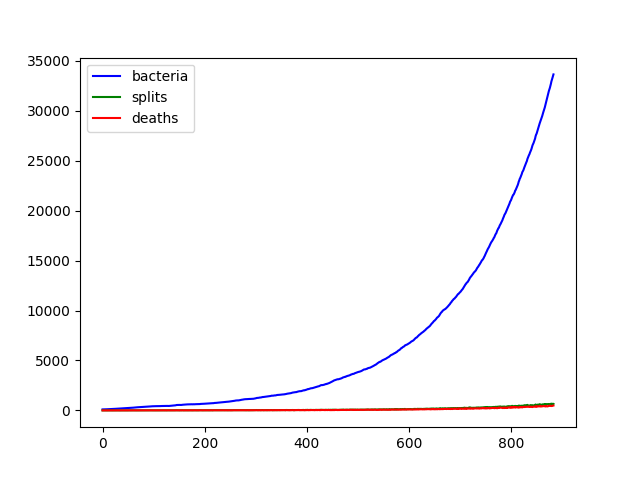
\includegraphics[width=1\textwidth]{Figure_3.png}
\caption{Evolution of total population}
\end{figure}

\begin{figure}[!h]
\centering
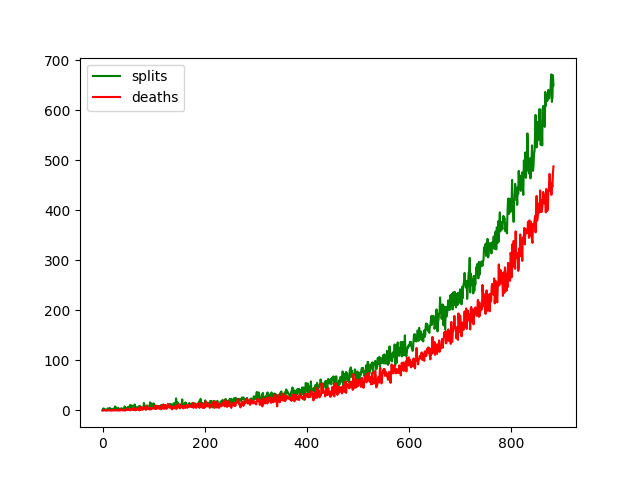
\includegraphics[width=1\textwidth]{Figure_1.png}
\caption{Evolution of the number of deaths and splits per unity of time}
\end{figure}

\begin{figure}[!h]
\centering
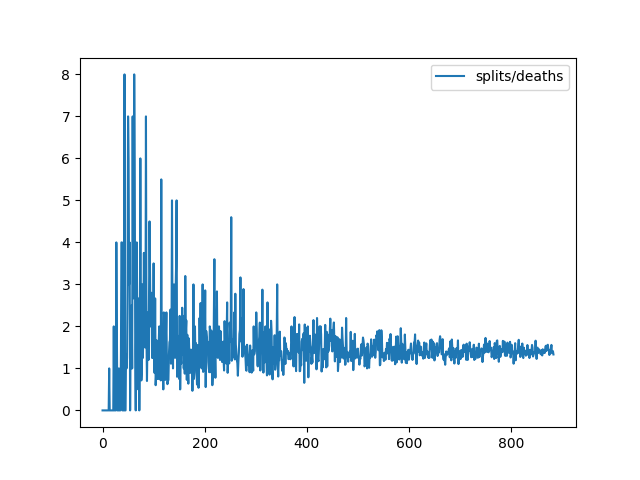
\includegraphics[width=1\textwidth]{Figure_4.png}
\caption{Evolution of the rate splits/deaths per unity of time}
\end{figure}

\end{document}